\documentclass[11pt]{article}
\usepackage{pictex, latexsym, graphicx,amsmath,amssymb,amsbsy,amsfonts,amsthm,verbatim}
\usepackage{fullpage,subfigure,hyperref}
\setlength{\parindent}{0em}

\def\vx{\mathbf{x}}
\def\vc{\mathbf{c}}
\def\vb{\mathbf{b}}
\def\vy{\mathbf{y}}

\begin{document}

%\thispagestyle{empty}
\title{
\begin{center}
\textbf{
\large Heuristic Methods for TSP
}
\end{center}}
\author{
Chan-Ching Hsu\\
\texttt{cchsu@iastate.edu}}
\date{\vspace{-5ex}}
\maketitle
%\vspace{1em}
\section{Problem}
The traveling salesman problem (TSP) asks the following question: Given a list of cities and the distances between each pair of cities, what is the shortest possible route that visits each city exactly once and returns to the original city? It is an NP-hard problem in combinatorial optimization, important in operations research and theoretical computer science.

Various heuristics and approximation algorithms, which quickly yield good solutions have been devised. Modern methods can find solutions for extremely large problems (millions of cities) within a reasonable time which are with a high probability just 2-3\% away from the optimal solution~\cite{TSP}.

%In this report, you will design heuristic methods to construct ``good'' solutions to the Traveling Salesman Problem where the nodes are points in the Euclidean plane and all distances are the standard Euclidean distance. This assignment is a combination algorithm and visualization assignment: every solution must be presented graphically. You should use some sort of plotting functionality to draw the best tour you can find using your techniques.

%You must implement one of each type of algorithm: \textbf{Initial Heuristic} and \textbf{Local Heuristic}. You will produce an initial tour using your initial heuristic and then improve it using your local heuristic.

%\begin{itemize}
%\item \textbf{Initial Heuristics}
%\begin{itemize}
%	\item Nearest Neighbor
%	\item Farthest Insertion
%	\item Nearest Insertion
%	\item Cheapest Insertion
%	\item Christofides' Heuristic
%\end{itemize}
%\item \textbf{Local Heuristics}
%\begin{itemize}
%	\item 2opt (2-switches)
%	\item 3opt (3-switches)
%	\item Lin-Kernighan ($\delta$-paths)
%\end{itemize}
%\end{itemize}

%\emph{Special Bonus Assignment:} If you implement an algorithm to produce Held-Karp Lower Bounds, then you will receive up to 10 extra points (out of the 30 total points). If you use such lower bounds, report the vector $\vy = (y_v)_{v\in V}$ and the 1-tree given by the lower bound. Plot the 1-tree and write the vertex values $y_v$ on the nodes. Report the relative difference between your upper and lower bounds.

%\vspace{1em}

%\textbf{\large Questions to Answer in Your Report}

%\textbf{Q1.} Which heuristics did you use?

%\textbf{Q2.} How specifically did you select which choices to make?

%\textbf{Q3.} What was the most difficult part of this assignment?


\section{Implementation}
The nearest neighbor algorithm was one of the first algorithms used to determine a solution to the traveling salesman problem. In it, the salesman starts at some city and then visits the city nearest to the starting city. From there he visits the nearest city that was not visited so far, etc., until all cities are visited, and the salesman returns to the start. The algorithm is described as below.
\begin{itemize}
  \item Nearest Neighbor Algorithm
\begin{enumerate}
  \item $V=\{1,\ldots,n-1\}$\quad\emph{* Vertices except for 0}.
  \item $U=\{0\}$\quad\quad\quad\quad\quad\quad\emph{* Vertex 0.}
  \item \textbf{while} $V$ not empty
  \item \quad $u=$ most recently added vertex to $U$
  \item \quad Find vertex $v$ in $V$ closet to $u$
  \item \quad Add $v$ to $U$ and remove $v$ from $V.$
  \item \textbf{endwhile}
  \item Ourput vertices in the order they were added to $U$
\end{enumerate}
\end{itemize}
Though usually rather bad, nearest neighbor tours only contain a few mistakes, but at the same time contain long segments connecting nodes with short edges. Therefore, such tours can serve as good starting tours for improvement methods.

The tours computed by the various construction heuristics initially are only of moderate quality. In general, improvement heuristics are characterized by a certain type of pf basic move to alter the current tour.

A 2-opt move consists of eliminating two edges and reconnecting the two resulting paths in a different way to obtain a new tour. There is only one way to reconnect the paths that yield a different tour. Among all pairs of edges whose 2-opt exchange decreases the length we choose the pair that gives the shortest tour. This procedure is then iterated until no such pair of edges is found. Two types of 2-opt heuristics are described as follows.



\begin{itemize}
  \item 2-OPT Heuristic
\begin{enumerate}
  \item $T=$ some starting tour
  \item noChange=true
  \item \textbf{repeat}
  \item \quad\textbf{foe all} possible edge-pairs in $T$
  \item \quad\quad $T'=$ tour by swapping end points in edge-pair
  \item \quad\quad\textbf{if} $T'<T$
  \item \quad\quad\quad $T=T'$
  \item \quad\quad\quad noChange=false
  \item \quad\quad\quad\textbf{break}\quad\emph{* Quit loop as soon as improvement is found}
  \item \quad\quad\textbf{endif}
  \item \quad\textbf{endfor}
  \item \textbf{until} noChange
  \item \textbf{return} $T$
\end{enumerate}
\end{itemize}

\begin{itemize}
  \item An Alternative: Find Best Tour with all Possible Swaps
\begin{enumerate}
  \item $T=$ some starting tour
  \item noChange=true
  \item \textbf{repeat}
  \item $T_{best}=T$
  \item \quad\textbf{foe all} possible edge-pairs in $T$
  \item \quad\quad $T'=$ tour by swapping end points in edge-pair
  \item \quad\quad\textbf{if} $T'<T_{best}$
  \item \quad\quad\quad $T_{best}=T'$
  \item \quad\quad\quad noChange=false
  \item \quad\quad\textbf{endif}
  \item \quad\textbf{endfor}
  \item \quad $T=T_{best}$
  \item \textbf{until} noChange
  \item \textbf{return} $T$
\end{enumerate}
\end{itemize}

Nearest neighbor algorithm is implemented to produce a initial tour and then the tour is improved by implementing the alternative 2-opt heuristic algorithm , which consider all possible swaps to find a better tour. Initial tours from my work were actually selected before performing 2-switches methods. All the possible initial tours were generated by choosing various starting vertex (first node added into $U$). The total length of each initial tour was computed and then compared; the shortest tour would be selected to conduct the local heuristic.

All the algorithm were developed in C Programming Language~\cite{C} and run on a ISU Engineering Linux server~\cite{Servers}. To plot tours in the solutions, I used gnuplot~\cite{Gnuplot}, which is a free, command-drive, interactive and data plotting program. As it is quick to implement the idea of the nearest neighbour algorithm, the 2-opt algorithm took me a long time to develop codes and verify the correctness. The most tricky part, I would say, is that one has to avoid accidently yield cycles after swapping; in addition, with the action of swapping, if the direction of the tour matters, the directions between effected vertices may need to be reversed accordingly.
\section{Solutions}
This section shows fundamentally the two results for each given instance, initial solutions and improved solutions.
\subsection{Instance I1}
With the solution from initial algorithm, I obtained the best initial tour and this tour doesn't have edges to swap in order to decrease the length. The best solution I have is illustrated in Fig. \ref{I1}.
\begin{figure}[ht]
\centering
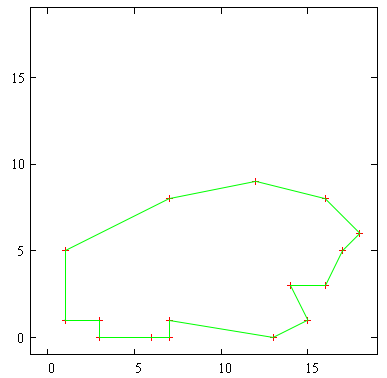
\includegraphics[width=3.2in]{I1}
\caption{Initial Result no Improvement to made}
\label{I1}
\end{figure}
\subsection{Instance I2}
Fig. \ref{I2initial} gives the best initial tour and Fig. \ref{I2local} shows the best improved tour by 2-opt moves.
\begin{figure}[ht]
\centering
\subfigure[Initial Result]{\label{I2initial}
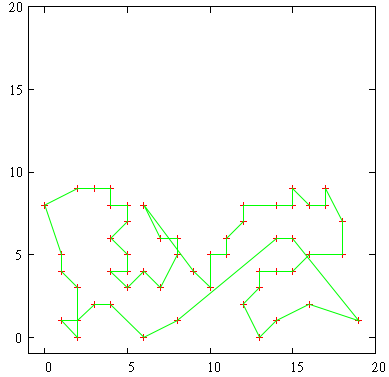
\includegraphics[width=2.8in]{I2initial}}
\subfigure[Local Optimization]{\label{I2local}
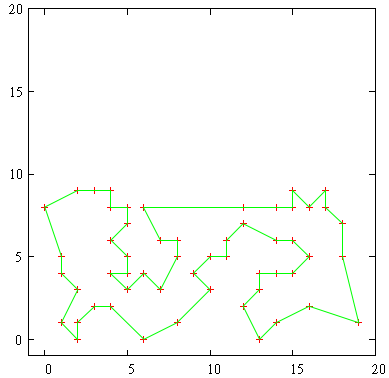
\includegraphics[width=2.8in]{I2local}}
\caption{The initial output and improved solution to I2}
\label{I2} %% label for entire figure
\end{figure}
\subsection{Instance I3}
Fig. \ref{I3initial} gives the best initial tour and Fig. \ref{I3local} shows the best improved tour by 2-opt moves.
\begin{figure}[!ht]
\centering
\subfigure[Initial Result]{\label{I3initial}
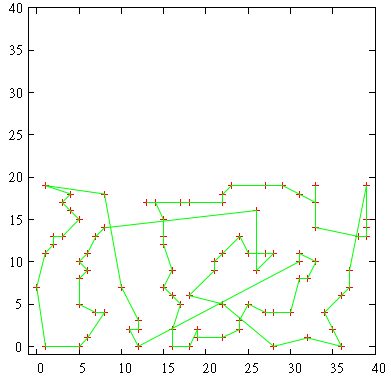
\includegraphics[width=2.8in]{I3initial}}
\subfigure[Local Optimization]{\label{I3local}
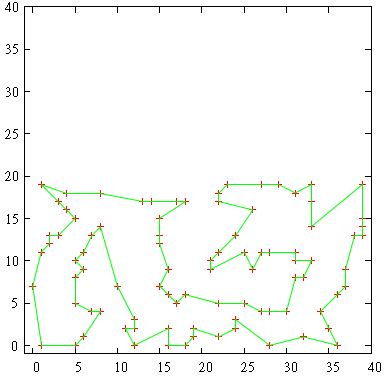
\includegraphics[width=2.8in]{I3local}}
\caption{The initial output and improved solution to I3}
\label{fig:Comparison} %% label for entire figure
\end{figure}
\subsection{Instance I4}
Fig. \ref{I4inital} gives the best initial tour and Fig. \ref{I4local} shows the best improved tour by 2-opt moves.
\begin{figure}[ht]
\centering
\subfigure[Initial Result]{\label{I4inital}
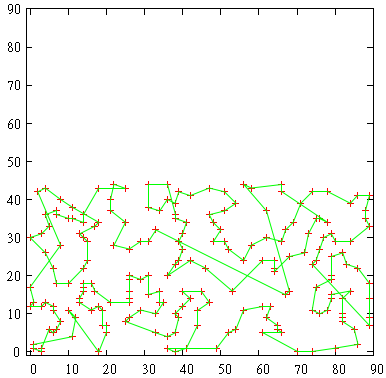
\includegraphics[width=2.8in]{I4inital}}
\subfigure[Local Optimization]{\label{I4local}
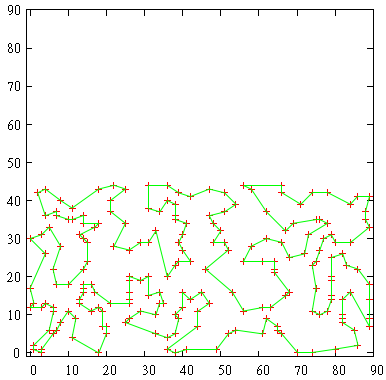
\includegraphics[width=2.8in]{I4local}}
\caption{The initial output and improved solution to I4}
\label{fig:Comparison} %% label for entire figure
\end{figure}

\begin{thebibliography}%\frenchspacing
%{
\small
\bibitem{TSP} "Traveling Salesman problem heuristics: leading methods, implementations and latest advances", \url{http://www.sciencedirect.com/science/article/pii/S0377221710006065}%
\bibitem{Gnuplot} gnuplot, \url{http://www.gnuplot.info/}
\bibitem{Servers} Linux Servers in College of Engineering, Iowa State University, \url{http://it.engineering.iastate.edu/remote/}
\bibitem{C} C Programming Language, \textit{Wikipedia}, \url{http://en.wikipedia.org/wiki/C_(programming_language)}
%}
\end{thebibliography}


\end{document} 